\subsection{Propuesta de diseño}
\label{propuesta}

\todo{Relacionar REST con nuestra propuesta. Utilizar como referencia el capítulo 6 de Fielding: \url{https://www.ics.uci.edu/~fielding/pubs/dissertation/evaluation.htm} y tomar la \autoref{fig:ejemplo-rest-nueva-arquitectura}}

\begin{figure}
  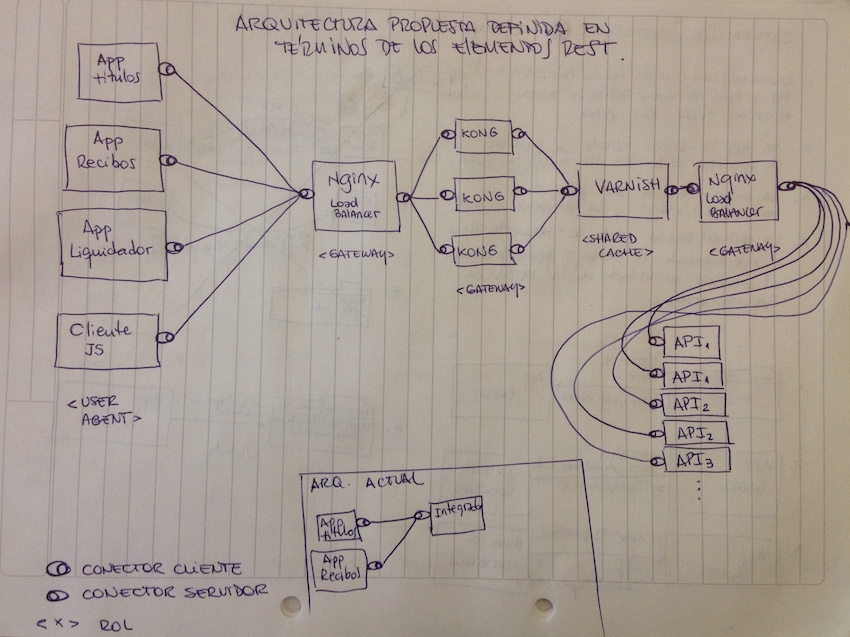
\includegraphics[width=\linewidth]{src/images/04-capitulo-4/nueva-arq-segun-rest.jpg}
  \caption{Visión \gls{acro:rest} de la nueva arquitectura propuesta}
  \label{fig:ejemplo-rest-nueva-arquitectura}
\end{figure}

\todo{Decir que se van a implementar como microservicios, aprovechando lo detallado en la \autoref{microservicios}.}

% ver en http://www.oreilly.com/programming/free/open-by-design.csp?download=yes&order=574386
% se puede sacar algo referente al opensource
% otro que puede servir Migrating to the Cloud?

Por lo expuesto anteriormente, se propone una arquitectura más desacoplada a la planteada con el Integrador, permitiendo de esta manera minimizar el costo del mantenimiento, desarrollo y simplificando su instalación (\eng{deployment}) en entornos de producción. Una solución basada en estándares que permita integrar sistemas heterogéneos, aceptando el hecho de que la mayoría de los sistemas legados que se encuentran en producción, se mantendrán y logrando de esta manera, que la infraestructura subyacente facilite la incorporación de cambios que puedan surgir como necesidades del \cespi y la \unlp.

El modelo de servicios facilita el acceso y consumo de la información a través de la red. Dado que los servicios son independientes y autónomos, pueden combinarse tantas veces como sea necesario de manera sencilla, generando nuevas aplicaciones que respondan a las necesidades en constante evolución de nuestra Casa de estudios. Esta posible agregación y combinación de servicios para resolver situaciones presentes y futuras convierten en una opción altamente beneficiosa el uso de una estrategia orientada a servicios, con el fin de crear servicios y aplicaciones compuestas que pueden existir con independencia de las tecnologías subyacentes\cite{microsoft2006}.

El resultado final es una nube, con conjunto de servicios y una creciente flota de aplicaciones dependientes de éstos, que se adapta fácilmente a los cambios.

En este capítulo profundizaremos la aplicación concreta de los conceptos vistos hasta aquí en el presente trabajo, explicando a través de los puntos mencionados en la \autoref{objetivo}.


\subsubsection{Redundancia y escalabilidad}

Cuando hablamos de escalabilidad, podemos basarnos en el modelo llamado \eng{scale cube}\cite{website:akfpartners-scale-cube}. Este modelo clasifica las distintas formas de escalar las aplicaciones en 3 sentidos, tomando como analogía las 3 dimensiones de un cubo:

\begin{itemize}
  \item \textbf{Escalar sobre el eje \textit{X}:} (\eng{X-axis scaling}, en inglés) Esta es la técnica más comúnmente utilizada para incrementar la disponibilidad de las aplicaciones. Consiste en el uso de instancias replicadas de la aplicación (idénticas a la original), ubicadas detrás de un balanceador de carga que reparte entre ellas el trabajo.
  \item \textbf{Escalar sobre el eje \textit{Y}:} (\eng{Y-axis scaling}, en inglés) Esta es una técnica que se encuentra en auge con el \textit{moméntum} que están teniendo los microservicios. Se basa en la descomposición funcional de la aplicación en un conjunto de servicios colaborativos, donde cada uno implementa un pequeño conjunto de funciones. En este caso, la disponibilidad se incrementa al separar en componentes más pequeñas la unidad funcional mayor que es la aplicación, dividiendo el trabajo independientemente entre ellas.
  \item \textbf{Escalar sobre el eje \textit{Z}:} (\eng{Z-axis scaling}, en inglés) En este enfoque se toma como base la replicación de instancias presente en \eng{X-axis scaling} y a esto se agrega una capa superior de abstracción que separa el conjunto de datos que cada instancia (o conjunto de éstas) atenderá, acorde a algún criterio lógico como puede ser el cliente que realice la petición (privilegiando unos clientes sobre otros).
\end{itemize}

\begin{figure}[H]
  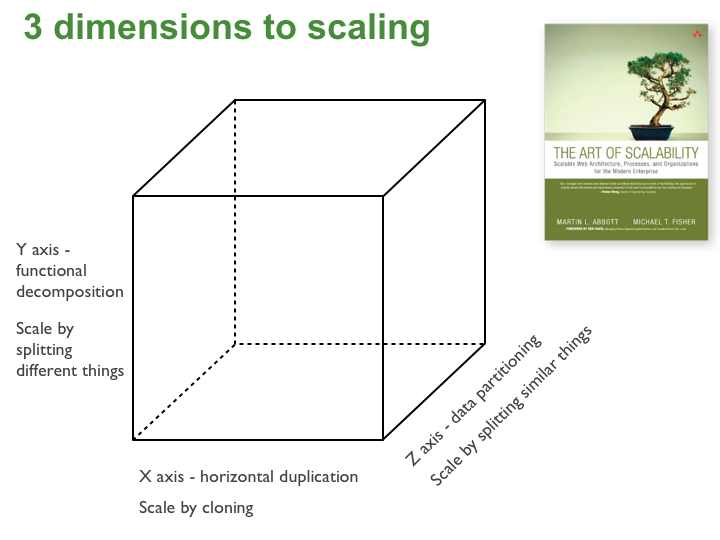
\includegraphics[width=\linewidth]{src/images/04-capitulo-4/scale_cube.jpg}
  \caption{El modelo de escalabilidad \eng{scale cube}}
  \label{fig:scale-cube}
\end{figure}

La arquitectura de servicios debe ser replicable y escalable. Para lograr esto cada \gls{acro:api} correrá en una instancia virtual independiente, de manera tal que la misma pueda ser replicada tantas veces como sea necesario (\eng{X-axis scaling}). El punto de acceso a esta arquitectura replicada será un balanceador de carga que servirá tanto para balancear la carga como \eng{failover}, dando continuidad a los servicios en caso de que alguna de las instancias replicadas fallen.

La característica fundamental de un balanceador de carga es ser capaz de distribuir las peticiones entrantes a un grupo de servidores (\eng{backends}) de acuerdo a un algoritmo de decisión y ponderación llamado \eng{scheduler}. Este algoritmo definirá cómo se toma la decisión de qué backend podría atender un requerimiento entrante, existiendo algunos simples (hacerlo de manera aleatoria o siguiendo un criterio ordenado por turnos como \eng{round robin}) y otros más sofisticados (que consideran otros factores como por ejemplo la carga de cada backend, su tiempo de respuesta promedio, el número de conexiones activas, la ubicación geográfica, etc.).

En su funcionamiento básico el balanceador de carga redirige las peticiones a alguno de los backends, el cual luego contesta al balanceador, para que finalmente sea el balanceador el que entregue la respuesta al cliente sin que este último sepa de la existencia de esta compleja arquitectura. Esta estructura transparente al cliente evita accesos directos entre éstos y los servidores que actúan como backend.

Como se mencionó anteriormente, el balanceador puede también ser usado como \eng{failover}, permitiendo que la falla de uno o más backends no afecten la disponibilidad del servicio. Los backends son monitoreados continuamente por el balanceador, cuando uno de estos falla el balanceador deja de enviar tráfico al backend caído. Luego cuando el backend vuelve a estar online el balanceador detecta esta situación y comienza a enviarle tráfico nuevamente.

Delante del balanceador se implementará una caché compartida utilizando \gls{db:varnish}, la misma evitará los accesos al balanceador, que puedan impactar de forma directa en alguna de las instancias replicadas de la \textit{API de Servicios} y \textit{API de Referencias}.

Según la RFC 7234\footnote{Este documento define las caches \gls{proto:http} y las cabeceras de control de cache permitidas en la versión \texttt{1.1} de ese protocolo\\\url{https://tools.ietf.org/html/rfc7234}}, una memoria cache almacena respuestas en pos de reducir el tiempo de respuesta y el consumo del ancho de banda. Asimismo, una memoria cache compartida es una cache que almacena respuestas para ser usadas por más de un usuario. Más adelante se tratará en detalle el uso de caches compartidas.

Como bien se indicó anteriormente, una cache compartida evitará los accesos a cualquiera de las instancias, ya sea de la \textit{API de Referencias} o la \textit{API de Servicios}, obteniendo mejores tiempos de respuesta así como tolerancia a fallos. Por ejemplo, podemos pensar en una aplicación (\textit{cliente A}) que accede al servicio \url{/academic_units} de la \textit{API de Referencias}. La petición es atendida por la \textit{API de Referencias}, donde el servicio devuelve todas la Unidades Académicas activas. Si más tarde otra aplicación (\textit{cliente B}), consulta la \gls{acro:api} por las Unidades Académicas, accediendo también al servicio \url{/academic_units} de la \textit{API de Referencias}, terminará obteniendo el mismo listado de Unidades Académicas. Como se puede apreciar, tenemos dos accesos a la \textit{API de Referencias} con idénticas respuestas, ambas procesadas por completo por uno o más backends. Esta situación puede evitarse con la inclusión de una cache compartida entre los diferentes clientes, logrando mejorar los tiempos de respuesta ya que la \textit{API de Referencias} recibirá únicamente un acceso, debiendo acceder y procesar los datos una única vez ya que el resto de las peticiones serán obtenidas desde la cache compartida.


\subsubsection{Desacoplamiento}

Para lograr el desacoplamiento, se propone desarrollar una \textit{API de Referencias} en la cual se implementarán los servicios necesarios que permitirán el acceso a los datos de referencia desde las distintas aplicaciones. El acceso a la \gls{acro:api} estará restringido a las direcciones IP de las aplicaciones (clientes) y al uso de un token, que se utilizará para validar el acceso a los servicios. Esta funcionalidad no será necesario desarrollarla, ya que esta capa de seguridad se implementará mediante el \gls{acro:esb}.

Para la solución planteada podemos observar las siguientes ventajas:

\begin{itemize}
  \item \textbf{Escalabilidad:} permite escalar horizontalmente (\eng{X-axis scaling}), es decir, en el hipotético caso que la \textit{API de Referencias} sea accedida por muchas aplicaciones, la misma podría replicarse en varias instancias, evitando la sobrecarga de cualquiera de ellas, al mismo tiempo que serviría como \eng{failover}.

  \item \textbf{Administración centralizada:} se centraliza la administración de los datos de referencia, evitando que la duplicidad se propague en cada aplicación que necesite utilizarlos.

  \item \textbf{Mantenimiento centralizado:} cuando hablamos de mantenimiento nos referimos a mejoras en la \gls{acro:api}, como por ejemplo, implementación de nuevos servicios, arreglo de errores, etc. Tener una \textit{API de Referencias} totalmente desacoplada de las aplicaciones que generan los datos permite actualizarla de forma más sencilla, evitando parar momentáneamente otras aplicaciones.

  \item \textbf{Agilización en el desarrollo:} otra de las ventajas que presenta este esquema, es la agilización en el desarrollo de nuevas aplicaciones. Ya no será necesario desarrollar el módulo que administra los datos de referencia, los mismos estarán en la \textit{API de Referencias} y se accederán a través de servicios.  De esta manera, evitamos duplicar código fuente para implementar esta funcionalidad, al mismo tiempo que acortamos los tiempos de desarrollo.
\end{itemize}

En segunda instancia, se deberán escribir de nuevo todas las \glspl{acro:api} que se encuentran actualmente en producción, esto es lo que llamaremos \textit{API de Servicios}. Para tal propósito, se utilizará el lenguaje de programación Ruby con el framework \nameref{soa:tecnologias:rails}, por los motivos que ya hemos expuesto en la \autoref{soa:tecnologias:para-servicios}. Esto dará origen a diferentes \textit{API de servicios}, que antes se encontraban implementados dentro de cada aplicación y acopladas a la misma, y ahora estarán implementados en una instancia virtual independiente.

De esta manera desacoplamos la lógica de la aplicación del acceso a los datos que se generan en la misma, permitiendo que esta solución escale horizontalmente, al igual que la \textit{API de Referencias}.

También se debe que tener en cuenta que esta solución permite independizarse del lenguaje en el que se desarrolló la aplicación: podemos desarrollar las aplicaciones en Ruby, PHP, JavaScript, Java o cualquier lenguaje, y la \gls{acro:api} separada en Ruby. Esto genera una capa de servicios en gran parte independiente de las aplicaciones, cuya única dependencia radica en el modelo de datos de cada aplicación, ya que si se modifica el modelo de la aplicación se deberá modificar de manera acorde el acceso a los datos, es decir los servicios.


\subsubsection{Simplicidad}

Es más simple que el anterior porque...

minimizar el costo del mantenimiento, desarrollo, testing, al mismo tiempo que se simplifica el deployment de los distintos entornos (desarrollo, testing y producción)

\subsubsection{Fault Tolerance}

Los sistemas distribuidos tienen potencialmente más fallos que los sistemas monolíticos, ya que en cada solicitud intervienen decenas (o cientos) de microservicios diferentes\cite[p.~48]{stin2015}. Es por esto que no resulta suficiente descomponer un sistema en componentes independientes; también hay que evitar que un fallo en uno de estos componenetes cause un fallo en cascada\cite[p.~4]{stin2015}.

Un fallo en cascada ocurre cuando un error en una capa interna provoca un fallo en la capa llamada\cite[p.~65]{nygard2007}. Mike Nygard describe en su libro ``Release It!''\cite{nygard2007} varios patrones tolerantes a fallos, de los cuales el mas popular es el \eng{Circuit Breaker}.

\begin{figure}[H]
  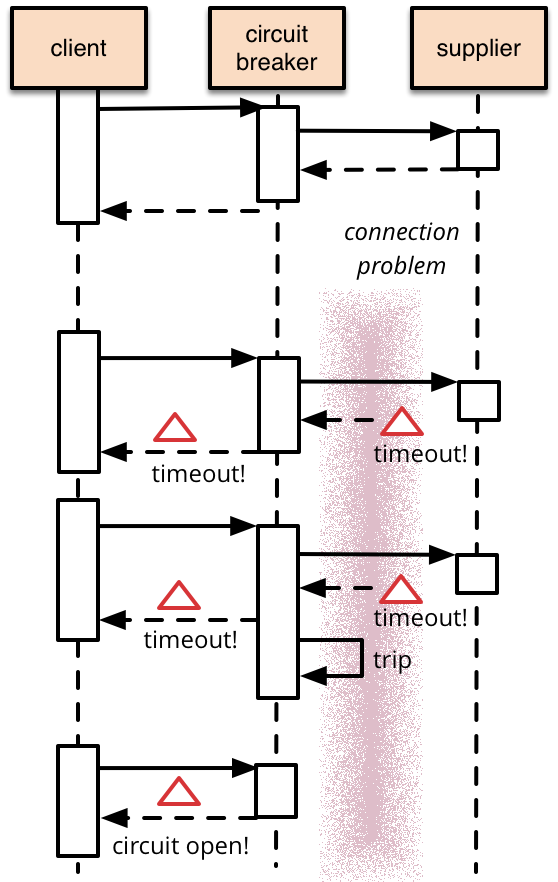
\includegraphics[width=\linewidth]{src/images/04-capitulo-4/circuit_breaker.png}
  \caption{Patrón de tolerancia a fallos \eng{Circuit Breaker}}
  \label{fig:circuit_breaker}
\end{figure}

Para implementar una infraestructura de servicios tolerante a fallos, los servicios estarán replicados en varias instancias virtuales y, como detallamos antes, delante de éstas se implementará un balanceador de carga, al mismo tiempo que se deberá trabajar en limitar el alcance de un fallo a nivel de servicio.

% ver si no es necesario sumar algo con respecto a los clientes

\subsubsection{Estandarización}

Según el diccionario de la Real Academia Española, un estándar es lo que sirve como tipo, modelo, norma, patrón o referencia. En nuestro caso, la estandarización es el proceso por el cual se establecen normas comunmente aceptadas que permiten la comunicación de diferentes aplicaciones.

Como mencionamos anteriormente, para cada aplicación que lo requiera se deberá implementar una \gls{acro:api} de acceso a datos propios generados localmente. Esta implementación se realizará basándose en la especificación \nameref{soa:tecnologias:json-api} detallada en la \autoref{soa:tecnologias:para-estructura}.

Esta estandarización facilitará el desarrollo de clientes que consuman información de los diferentes servicios de las \glspl{acro:api}, ya que definen con reglas que especifican cómo se podrá acceder a los datos, cuál será su estructura de respuesta, e incluso asisten en lograr independencia del lenguaje con el que se escriban estos clientes, quienes simplemente deben respetar las especificaciones para implementar el acceso a los servicios.
